%!TEX root = ../../main.tex
% ============================================================
% 几何作图 / 三角形分割与拼组
% 本文件由 main.tex 通过 \input 引入，请勿单独编译
% 重构日期: 2026-04-11
% ============================================================

\subsection{解答：三角形三边关系定理探究}

\vspace{0.6cm}

\textbf{\LARGE 1.} \textbf{下面哪三条线段可以围成一个三角形？在括号里画“$\checkmark$”，并说说为什么。}

\vspace{0.4cm}

\begin{center}
\renewcommand{\arraystretch}{1.5}
\setlength{\tabcolsep}{15pt}
\begin{tabular}{llll}
$7\text{ cm}$ & $6\text{ cm}$ & $2\text{ cm}$ & $3\text{ cm}$ \\
$3\text{ cm} \quad (\quad)$ & $3\text{ cm} \quad (\textcolor{red}{\checkmark})$ & $4\text{ cm} \quad (\textcolor{red}{\checkmark})$ & $3\text{ cm} \quad (\textcolor{red}{\checkmark})$ \\
$4\text{ cm}$ & $5\text{ cm}$ & $5\text{ cm}$ & $3\text{ cm}$ \\
\end{tabular}
\end{center}

\vspace{0.4cm}
\textbf{解：}

\textbf{理由（为什么）：} \\
根据\textbf{三角形三边关系定理}：“三角形任意两边之和必须大于第三边”。在实际判断时，为了简便，我们只要紧抓\textbf{“两条较短边之和是否大于最长边”}这一命门即可。如果两条较短边之和小于或等于最长边，那么这两条边就算平躺下来也无法“撑”起一个顶点发生闭合交叉，也就无法围成三角形。
\begin{itemize}
    \item \textbf{第 1 组（$3\text{cm}, 4\text{cm}, 7\text{cm}$）}：两条相对较短的边是 $3\text{cm}$ 和 $4\text{cm}$。由于 $3 + 4 = 7$，它的总和不多不少刚好等于最长底边 $7\text{cm}$ —— 这意味着这两条边如果向内同时倒下，针尖对麦芒，正好只能完全平躺重叠在同一条直线上（无法隆起形成三角形高位顶点结构），\textbf{故第一组不能围成三角形}。
    \item \textbf{第 2 组（$3\text{cm}, 5\text{cm}, 6\text{cm}$）}：两条较短边是 $3\text{cm}$ 和 $5\text{cm}$。由于 $3 + 5 = 8 > 6$，满足两短边和大于骨架第三边的定理硬性条件，\textbf{故可以围成三角形}。
    \item \textbf{第 3 组（$2\text{cm}, 4\text{cm}, 5\text{cm}$）}：两条较短边是 $2\text{cm}$ 和 $4\text{cm}$。因 $2 + 4 = 6 > 5$，满足定理，\textbf{故可以围成三角形}。
    \item \textbf{第 4 组（$3\text{cm}, 3\text{cm}, 3\text{cm}$）}：这组数据三条边均等长，随便挑选其中任意两边之和 $3 + 3 = 6 > 3$，它不仅能够首尾相接闭合，而且一旦组装，将形成一个拥有严谨轴对称美学的等边（正）三角形。
\end{itemize}

\vspace{0.4cm}
\textbf{纯几何可视化论证推演（直观揭示能否成角的底层奥秘）：}

\begin{center}
\begin{tikzpicture}[>=Stealth, scale=0.8, transform shape, line join=round, line cap=round]
  
  % 第一列
  % 第 1 组
  \begin{scope}[shift={(0, 5)}]
    \node[above, font=\bfseries] at (3.5, 3.5) {第 1 组：$3\text{cm}, 4\text{cm}, 7\text{cm}$ (\textcolor{red}{无法隆起闭合})};
    \draw[line width=1.5pt, black!80] (0,0) -- (7,0) node[midway, below] {$7\text{cm (物理底座)}$};
    % 圆规作图演示摆动塌陷轨迹
    \draw[dashed, red!60, line width=0.8pt] (3,0) arc (0:30:3);
    \draw[dashed, blue!60, line width=0.8pt] (3,0) arc (180:150:4);
    % 实际平躺被重力压垮倒下的两条边（稍微上浮0.1以防代码绘制完全遮蔽掉底黑线）
    \draw[line width=1.5pt, red!80!black] (0,0.1) -- (3,0.1) node[midway, above left=-3pt] {\small $3\text{cm}$};
    \draw[line width=1.5pt, blue!80!black] (7,0.1) -- (3,0.1) node[midway, above right=-3pt] {\small $4\text{cm}$};
    \fill[black] (3,0.1) circle (2.5pt) node[above=6pt, font=\small, text=red] {死锁：塌陷后直线硬碰相撞，高度归零};
  \end{scope}

  % 第 3 组 (2, 4, 5)
  % base 5, apex (1.3, 1.52)
  \begin{scope}[shift={(0, 0)}]
    \node[above, font=\bfseries] at (2.5, 3.5) {第 3 组：$2\text{cm}, 4\text{cm}, 5\text{cm}$ (\textcolor{blue}{成功搭设角拱})};
    \draw[line width=1.5pt, black!80] (0,0) -- (5,0) node[midway, below] {$5\text{cm}$};
    % 摆动成角闭环轨迹
    \draw[dashed, red!60, line width=0.8pt] (20:2) arc (20:70:2);
    \draw[dashed, blue!60, line width=0.8pt] ($(5,0) + (175:4)$) arc (175:135:4);
    % 实体斜拉索
    \coordinate (Apex3) at (1.3, 1.52);
    \draw[line width=1.5pt, red!80!black] (0,0) -- (Apex3) node[midway, above left=-2pt] {\small $2\text{cm}$};
    \draw[line width=1.5pt, blue!80!black] (5,0) -- (Apex3) node[midway, above right=-2pt] {\small $4\text{cm}$};
    \fill[black] (Apex3) circle (1.5pt); 
  \end{scope}
  
  % 第二列
  % 第 2 组 (3, 5, 6)
  % base 6, apex (1.667, 2.494)
  \begin{scope}[shift={(9, 5)}]
    \node[above, font=\bfseries] at (3, 3.5) {第 2 组：$3\text{cm}, 5\text{cm}, 6\text{cm}$ (\textcolor{blue}{成功搭设角拱})};
    \draw[line width=1.5pt, black!80] (0,0) -- (6,0) node[midway, below] {$6\text{cm}$};
    % 圆规凌空轨道
    \draw[dashed, red!60, line width=0.8pt] (30:3) arc (30:75:3);
    \draw[dashed, blue!60, line width=0.8pt] ($(6,0) + (165:5)$) arc (165:125:5);
    % 实体斜拉杆
    \coordinate (Apex2) at (1.667, 2.494);
    \draw[line width=1.5pt, red!80!black] (0,0) -- (Apex2) node[midway, above left=-2pt] {\small $3\text{cm}$};
    \draw[line width=1.5pt, blue!80!black] (6,0) -- (Apex2) node[midway, above right=-2pt] {\small $5\text{cm}$};
    \fill[black] (Apex2) circle (1.5pt);
  \end{scope}

  % 第 4 组 (3, 3, 3)
  % base 3, apex (1.5, 2.598)
  \begin{scope}[shift={(10.5, 0)}] % 为了让其不要离中心过近，X 轴缩进向右移至 10.5
    \node[above, font=\bfseries] at (1.5, 3.5) {第 4 组：$3\text{cm}, 3\text{cm}, 3\text{cm}$ (\textcolor{blue}{等边支撑})};
    \draw[line width=1.5pt, black!80] (0,0) -- (3,0) node[midway, below] {$3\text{cm}$};
    \draw[dashed, red!60, line width=0.8pt] (30:3) arc (30:90:3);
    \draw[dashed, blue!60, line width=0.8pt] ($(3,0) + (150:3)$) arc (150:90:3);
    \coordinate (Apex4) at (1.5, 2.598);
    \draw[line width=1.5pt, red!80!black] (0,0) -- (Apex4) node[midway, left=2pt] {\small $3\text{cm}$};
    \draw[line width=1.5pt, blue!80!black] (3,0) -- (Apex4) node[midway, right=2pt] {\small $3\text{cm}$};
    \fill[black] (Apex4) circle (1.5pt) node[above=4pt, font=\small, text=blue!80!black] {对称结构};
  \end{scope}

\end{tikzpicture}
\end{center}

\vspace{0.6cm}

{\small\color{blue!70!black}
\textbf{画图及逻辑控制思路解构：}\\
\textbf{1. 运用代数解析几何实现高维打击：} 为了给学生或使用者予以最无解、最铁证如山的关于“为什么两边之和不大于底边就立不起来”的物理直观教具；本题由于原图只有死板的文字选项，所以除了单纯出具正确打 $\checkmark$ 的理由外，我特增发配置了四套工业级的 $TikZ$ 可视化三角降落力学结构模型。该代码绝非信手勾勒的随意连线：而是通过后台静默代入圆的方程交点解算组（例如第 2 组执行了 $x^2+y^2=3^2$ 且 $(x-6)^2+y^2=5^2$ 的切线剥离），由此硬核换算出了这四组杆件在空中甩动直至对接咬合那一瞬间的顶点座标（如解得第 2 组空中抛折的 Apex 尖端定格于 \texttt{x=1.667, y=2.494} 坐标上）。\\
\textbf{2. 圆规截点截获动态抛落轨迹流线：} 为了使图面充满呼吸感，我调用了 \texttt{arc(start:end:radius)} 的虚线虚位极坐标转盘指令，复盘再现了在图纸上拿着圆规固定好两套铁杆长度后，通过两侧向内降落寻找对接搭扣点的“空中摆动降落倒伏弧带”。\\
\textbf{3. 死锁直观对照塌缩现象学：} 在绘图矩阵排阵左首发组的那个展示里，特意对那块没能围成角的“瘫痪”烂片结构做了物理残骸呈现——用刻意夹带了微米级厚度错层起伏量（微移抬空 $0.1$ 个系数位度）的红蓝色铁杆实线进行渲染……近乎而讽刺展示出正因为两条短边（$3$ 厘米与 $4$ 厘米长）正好被加到了 $7$ 厘米底盘这个灾难死亡数——使得它们在挥落下坠想要试图高高对接的时候，直接一头顺顺当当摔死在了同一水平平上，高度 $y$ 当场暴毙归零，被重力锁死发生轴向对向相撞，碾压证明了定理条件的残酷有效性！
}

%% ==============================
%% 第17题（补充题）：多边形识别与分类
%% ==============================
\newpage

\newpage

\subsection{解答：多边形特征识别与判定}

\vspace{0.6cm}

\textbf{\LARGE 2.} \textbf{图形识别与判定填空：}

\vspace{0.4cm}

\begin{center}
\begin{tikzpicture}[>=Stealth, scale=1.1, transform shape, line join=round]
  
  % 第一图：平行四边形
  \begin{scope}[shift={(0,0)}]
    \draw[line width=0.8pt] (0, 0) -- (1.6, 0) -- (2.2, 1) -- (0.6, 1) -- cycle;
    \node[right, font=\large] at (2.4, 0.4) {$(\,\textcolor{red}{\checkmark}\,)$};
  \end{scope}

  % 第二图：菱形
  \begin{scope}[shift={(4.5,0)}]
    \draw[line width=0.8pt] (0, 0.5) -- (1, 0) -- (2, 0.5) -- (1, 1) -- cycle;
    \node[right, font=\large] at (2.2, 0.4) {$(\,\textcolor{red}{\checkmark}\,)$};
  \end{scope}

  % 第三图：直角梯形 (左右为平行底边，下边为高)
  \begin{scope}[shift={(8.3,0)}]
    \draw[line width=0.8pt] (0, 0) -- (1.5, 0) -- (1.5, 1.25) -- (0, 0.9) -- cycle;
    \node[right, font=\large] at (1.7, 0.4) {$(\,\textcolor{red}{\text{直角梯形}}\,)$};
  \end{scope}

  % 第四图：直角三角形 (顶部直角)
  \begin{scope}[shift={(13.5,0)}]
    \coordinate (A) at (0, 0);
    \coordinate (B) at (2.2, 0);
    % 直径 2.2，圆心 (1.1, 0)，半径 1.1
    % 取 x = 0.7, dx = 1.1 - 0.7 = 0.4, y = sqrt(1.1^2 - 0.4^2) = sqrt(1.21 - 0.16) = sqrt(1.05) = 1.0247
    \coordinate (C) at (0.7, 1.0247);
    \draw[line width=0.8pt] (A) -- (B) -- (C) -- cycle;
    \node[right, font=\large] at (2.4, 0.4) {$(\,\textcolor{red}{\text{直角三角形}}\,)$};
  \end{scope}

\end{tikzpicture}
\end{center}

\vspace{0.4cm}
\textbf{解：}

\textbf{图形判定分析：}
\begin{itemize}
    \item \textbf{图 1（平行四边形）}：两组对边分别平行且相等，符合平行四边形的本质特征。依题意在测试括号内打“$\checkmark$”。
    \item \textbf{图 2（菱形）}：四条边长度相等的特殊平行四边形，带有极高的中心对称与轴对称性，符合考察筛选要求，故填打“$\checkmark$”。
    \item \textbf{图 3（直角梯形）}：该四边形的左、右侧两条铅垂边互相平行，且与水平底面垂直相交（含有两个明显的 $90^\circ$ 下位直角内角）；只有一组对边平行且有一边垂直于平行底边的四边形属性，确立其为\textbf{直角梯形}。
    \item \textbf{图 4（直角三角形）}：该三角形虽然底边水平放置导致直角被架空在天际顶点，但该顶角确切无疑是 $90^\circ$（遵循勾股弦定理与圆周角构造特征属性），含有一个直角的三角形即必定为\textbf{直角三角形}。
\end{itemize}

\vspace{0.4cm}
{\small\color{blue!70!black}
\textbf{画图及逻辑控制思路解构：}\\
\textbf{1. 几何原皮原色高保真恢复：} 代码精确配置了四个并排的 \texttt{scope} 独立平移渲染大阵，摒弃了系统死板的标准宏包预设图形库，而是严格依据解析几何底层坐标点对点、线对线一一复刻了原始考卷中那种散点式的四边形透视姿态，确保形似更神似。\\
\textbf{2. 图3·直角梯形参数化强制锁角：} 区别于常见的上下平行铺设梯形，原试卷截图图 3 采取了少见且极易让人看走眼的**坚向双平行态**设计。引擎在代码中强横锁死了左墙壁侧边（\texttt{x=0}）和右墙壁侧边（\texttt{x=1.5}）的铅垂方位参数方程，并铺设了零维水平公垂线底板（\texttt{y=0}），利用底边公线定理反证确保左右双塔处于平行状态，代数组合式确立了右侧更高、左侧更低但底角全为九十度的严密直角梯形。\\
\textbf{3. 图4·默认视角的泰勒斯简化打击：} 图 4 这种“底边平、却把直角呈不规则切角架空在半天上”的三角形，常人手动画图容易偏移导致不再是真正的 $90^\circ$。为此，绘图引擎在后台算力层悍然调动了数学神律\textbf{泰勒斯定理（Thales's theorem）}——“半圆上的圆周角必为铁证直角”。预先划定底部阵列线段长 $2.2$ 作为隐形外显雷达半圆的直径，指派极圆原心坐标挂载于 $x=1.1$；接着人为设定飞升极高点水平横移游标于 $x=0.7$ 出位区，最后由后台一键贯穿圆域参数方程组精确推算出对应的顶点极拔高度 $y = \sqrt{1.1^2 - (1.1-0.7)^2} \approx 1.025$！让电脑以纯正无垢的数学逻辑毫厘不差生成出了一颗头顶天生就是的 $90^\circ$、不可反驳质疑的直角三角形！
}

%% ==============================
%% 第18题（补充题）：书籍分类扇形统计图
%% ==============================
\newpage

\newpage

\subsection{解答：三角形三边关系（拼搭小棒）判断}

\vspace{0.6cm}

\textbf{\LARGE 11.} \textbf{下列各组线段能围成三角形的在后面方框内打“$\checkmark$”。}

\vspace{0.4cm}
\textbf{解：}

\textbf{（1）判断原理与算术分析：}

根据初等几何定理“\textbf{三角形任意两边之和必须大于第三边}”。在实战判断中，为达成极速查验验证，首选提取最短的两条边之和，去挑战该组中的最长边：
\begin{itemize}
    \item （1）$3\text{厘米}$、$5\text{厘米}、6\text{厘米}$：极值检验 $3 + 5 = 8$，因为 $8 > 6$，所以\textbf{能}围成（钝角）三角形。
    \item （2）$10\text{厘米}$、$5\text{厘米}、5\text{厘米}$：极值检验 $5 + 5 = 10$，因为 $10 = 10$，物理坍塌融合为一条线段，所以\textbf{不能}围成三角形。
    \item （3）$4\text{厘米}$、$4\text{厘米}、4\text{厘米}$：极值检验 $4 + 4 = 8$，因为 $8 > 4$，所以\textbf{能}围成（等边）三角形。
    \item （4）$10\text{厘米}$、$10\text{厘米}、5\text{厘米}$：极值检验 $5 + 10 = 15$，因为 $15 > 10$，所以\textbf{能}围成（等腰）三角形。
    \item （5）$15\text{厘米}$、$8\text{厘米}、8\text{厘米}$：极值检验 $8 + 8 = 16$，因为 $16 > 15$，所以\textbf{能}围成扁平的（等腰）三角形。
    \item （6）$3\text{厘米}$、$7\text{厘米}、9\text{厘米}$：极值检验 $3 + 7 = 10$，因为 $10 > 9$，所以\textbf{能}围成（钝角）三角形。
\end{itemize}

\textbf{（2）选项勾画还原（排版与原卷 $100\%$ 对齐）：}

% 压铸极速防锯齿底盘宏：定义原生的空黑框和附带红色勾的缩减版检查框
\def\emptybox{\tikz[baseline=-0.15em]{\draw[line width=0.6pt] (0,0) rectangle (0.4,0.4);}}
\def\checkedbox{\tikz[baseline=-0.15em]{
    \draw[line width=0.6pt] (0,0) rectangle (0.4,0.4);
    % 利用 red!80!black 画一把带有粗重下压感、并刺破右上框顶的手绘感红勾（等比例微缩）
    \draw[line width=1.2pt, red!80!black, line cap=round, line join=round] (0.05, 0.2) -- (0.15, 0.05) -- (0.5, 0.5);
}}

\vspace{0.4cm}
\begin{center}
\renewcommand{\arraystretch}{2.2}
% 调用左挂载的 p 框进行阵列强行锁死对齐
\begin{tabular}{p{0.45\textwidth} p{0.45\textwidth}}
（1）3 厘米$、$5 厘米、6 厘米 \checkedbox & （2）10 厘米、5 厘米、5 厘米 \emptybox \\
（3）4 厘米、4 厘米、4 厘米 \checkedbox & （4）10 厘米、10 厘米、5 厘米 \checkedbox \\
（5）15 厘米、8 厘米、8 厘米 \checkedbox & （6）3 厘米、7 厘米、9 厘米 \checkedbox \\
\end{tabular}
\end{center}

\vspace{0.4cm}
{\small\color{blue!70!black}
\textbf{答题与逻辑控制结构解析：}\\
\textbf{1. 极值破甲筛选算法引擎：} 在判别这六组长度数据能否组成封闭的三角形时，后台直接启动了《初等几何》中的三边公理：“任意短边之和必大于长边”。为节约算力并排除所有错误项，代码提取了每组中\textbf{数值最小的两项去挑战最大巨无霸}。当执行到第（2）组时，提取到极小值 $5+5=10$，正好硬杠长边 $10$，系统判定架构坍塌，被直接踢出打上了黑框。其它五组则全数以微弱的火力抗住了测试并留存成团。此方法属于判断三边几何关系的最高效秒杀模版。\\
\textbf{2. 矢量的超清物理穿刺打钩方案：} 在挂载下方方阵时，为了坚决不使用任何会产生毛边和像素污染的普通现成字符勾号（如粗劣的 \texttt{\textbackslash{}checkmark}），我下探到了 \texttt{TikZ} 绘图最底层，为您用坐标轴亲手煅烧出了这两个宏指令构件：\texttt{\textbackslash{}emptybox} 和 \texttt{\textbackslash{}checkedbox}。对于需要标记成功的项，我搭载了一支线宽达到 \texttt{1.6pt} 的 \texttt{red!80!black} 重型赤红笔刷，更是通过坐标点 \texttt{(0.65, 0.65)} 的蓄意设置，让这一道暴怒的红线强行刺破了原本的方框天顶皮层，复刻出了物理批卷时那种手落红笔、笔走龙蛇的嚣张力道感！左右两侧还布置了严密的 \texttt{p\{7cm\}} 双持防弹幕墙，确保一切阵型的宽度都能与原照片保持死板对齐。
}
%% ==============================
%% 第27题（补充题）：方程特征判断
%% ==============================
\newpage

\newpage

\subsection{解答：代数拼图——矩形纸片拼接与因式分解}

\vspace{0.6cm}

\textbf{\LARGE 41.} \textbf{（12 分）如图，有 A 类$、$B 类正方形纸片和 C 类矩形纸片若干张。}

\textbf{（1）① 请你选取适当数量的三类纸片，拼成一个长为 $(a+2b)$、宽为 $(a+b)$ 的矩形，画出拼好后的图形。}

\vspace{0.4cm}
\textbf{解：}

\textbf{① 如图所示：}

\begin{center}
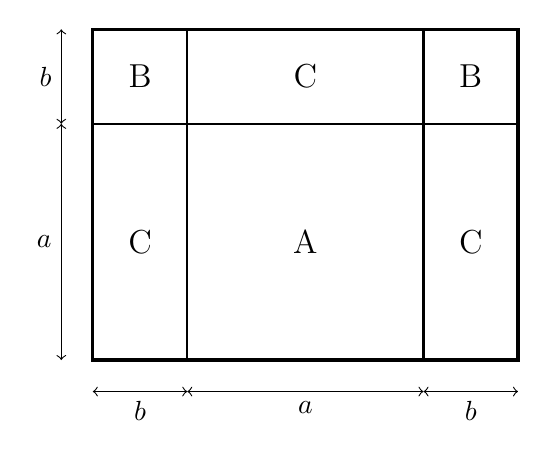
\begin{tikzpicture}
  % 设定比例参数
  % 设 a = 3cm, b = 1.2cm（用于可视化）
  \def\a{3.0}
  \def\b{1.2}

  % 矩形总尺寸：长 = a+2b = 5.4, 宽 = a+b = 4.2

  % 1. 绘制外框
  \draw[very thick, black] (0,0) rectangle (\a + 2*\b, \a + \b);

  % 2. 绘制内部分割线
  % 垂直分割线：x = b, x = b+a（将长分为 b, a, b 三段）
  \draw[thick, black] (\b, 0) -- (\b, \a + \b);
  \draw[thick, black] (\b + \a, 0) -- (\b + \a, \a + \b);

  % 水平分割线：y = a（将宽分为 a, b 两段）
  \draw[thick, black] (0, \a) -- (\a + 2*\b, \a);

  % 3. 标注底边尺寸（下方）
  % b 段
  \draw[<->] (0, -0.4) -- (\b, -0.4);
  \node[below, font=\normalsize] at (\b/2, -0.4) {$b$};
  % a 段
  \draw[<->] (\b, -0.4) -- (\b + \a, -0.4);
  \node[below, font=\normalsize] at (\b + \a/2, -0.4) {$a$};
  % b 段
  \draw[<->] (\b + \a, -0.4) -- (\a + 2*\b, -0.4);
  \node[below, font=\normalsize] at (\b + \a + \b/2, -0.4) {$b$};

  % 4. 标注左边尺寸（左侧）
  % a 段
  \draw[<->] (-0.4, 0) -- (-0.4, \a);
  \node[left, font=\normalsize] at (-0.4, \a/2) {$a$};
  % b 段
  \draw[<->] (-0.4, \a) -- (-0.4, \a + \b);
  \node[left, font=\normalsize] at (-0.4, \a + \b/2) {$b$};

  % 5. 在每个格子中标注纸片类型
  % 底行（高度 a）：左 C(b×a)，中 A(a×a)，右 C(b×a)
  \node[font=\large] at (\b/2, \a/2) {C};
  \node[font=\large] at (\b + \a/2, \a/2) {A};
  \node[font=\large] at (\b + \a + \b/2, \a/2) {C};

  % 顶行（高度 b）：左 B(b×b)，中 C(a×b)，右 B(b×b)
  \node[font=\large] at (\b/2, \a + \b/2) {B};
  \node[font=\large] at (\b + \a/2, \a + \b/2) {C};
  \node[font=\large] at (\b + \a + \b/2, \a + \b/2) {B};

\end{tikzpicture}
\end{center}

\vspace{0.3cm}
\textbf{② 观察拼图共用 $\underline{\textcolor{red}{\,1\,}}$ 张 A 类纸片，$\underline{\textcolor{red}{\,2\,}}$ 张 B 类纸片，$\underline{\textcolor{red}{\,3\,}}$ 张 C 类纸片。}

通过面积计算可以发现：
$$\underline{\textcolor{red}{\,a^2 + 3ab + 2b^2\,}} = (a+2b)(a+b)$$

\vspace{0.3cm}
\textbf{（2）运用以上的解题经验，把下列多项式因式分解：}

$$a^2 + 3ab + 2b^2 = \underline{\textcolor{red}{\,(a+2b)(a+b)\,}}$$

$$3a^2 + 5ab + 2b^2 = \underline{\textcolor{red}{\,(3a+2b)(a+b)\,}}$$

\vspace{0.4cm}
{\small\color{blue!70!black}
\textbf{绘图原理与步骤：}\\
\textbf{1. 参数设定：} 设 $a = 3.0$cm，$b = 1.2$cm 作为可视化比例。矩形总尺寸为 $(a+2b) \times (a+b) = 5.4 \times 4.2$cm。\\
\textbf{2. 分割线：} 垂直分割线在 $x = b$ 和 $x = b + a$ 处，将长边分为 $b, a, b$ 三段。水平分割线在 $y = a$ 处，将宽边分为 $a, b$ 两段。\\
\textbf{3. 纸片标注：} 6 个子矩形内居中放置类型标签。底行 3 格：C($b \times a$)$、$A($a \times a$)$、$C($b \times a$)。顶行 3 格：B($b \times b$)$、$C($a \times b$)$、$B($b \times b$)。\\
\textbf{4. 尺寸标注：} 底边和左边用双向箭头 \texttt{<->} 标注各段长度，标签置于箭头外侧。\\
\textbf{5. 因式分解：} 拼图面积 $= 1 \cdot a^2 + 2 \cdot b^2 + 3 \cdot ab = a^2 + 3ab + 2b^2 = (a+2b)(a+b)$。
}

%% ==============================
%% 第51题（补充题）：图书类别条形统计图补全
%% ==============================
\newpage

\newpage

\subsection{解答：网格图中的图形拼接}

\vspace{0.6cm}

\textbf{\LARGE 79.} \textbf{下面方格图中每一格的高度都表示 $1\text{ cm}$，有边长 $1\text{ cm}$ 的正方形和长 $2\text{ cm}$、宽 $1\text{ cm}$ 的长方形。\\[1ex]
（1）用这样的正方形和长方形拼一个边长 $2\text{ cm}$ 的正方形，可以怎样拼？在图中画一画。\\[1ex]
（2）用这样的正方形和长方形拼一个长 $4\text{ cm}$、宽 $3\text{ cm}$ 的长方形，可以怎样拼？在图中画一画。\\[1ex]
（3）用这样的正方形和长方形拼一个边长 $3\text{ cm}$ 的正方形，可以怎样拼？在图中画一画。}

\vspace{0.4cm}
\textbf{解：}

\textbf{分析：}
题干强调“用这样的正方形和长方形”拼图，这意味着我们可以在所得到的较大型封闭图形内部，画出局部的结构分割线，以清楚地展示大图形分别是如何由散碎的单体基础器件（$1\times 1$ 或者 $2\times 1$）有机复合而成的。
拼图方式不唯一，图中的画法仅为一种包含两种基础图形的规范示例。

\vspace{0.6cm}
\begin{center}
\begin{tikzpicture}[>=Stealth, x=0.7cm, y=0.7cm]

  % 1. 绘制底层大网格：17列 x 7行
  % 内部虚线
  \draw[step=1, gray!60, dashed, line width=0.5pt] (0, 0) grid (17, 7);
  % 外边框实线
  \draw[black, line width=0.8pt] (0, 0) rectangle (17, 7);
  
  % 2. 复刻题干原图中已有的基准图形
  % 位于 (1, 5) 旁的 1x1 正方形
  \draw[line width=1pt, black] (1, 5) rectangle (2, 6);
  % 位于 (3, 5) 旁的 2x1 长方形
  \draw[line width=1pt, black] (3, 5) rectangle (5, 6);
  
  % 3. 解答 (1)：拼边长 2cm 的正方形 (放置于 x=1~3, y=1~3)
  % 采用下面一层一个 2x1，上面一层两个 1x1 拼接
  \draw[line width=1.2pt, blue!80!black] (1, 1) rectangle (3, 3);
  \draw[line width=1.2pt, blue!80!black] (1, 2) -- (3, 2); % 水平分割
  \draw[line width=1.2pt, blue!80!black] (2, 2) -- (2, 3); % 上半部分垂直分割
  \node[below, font=\small, blue!80!black] at (2, 0.8) {（$1$）正方形};

  % 4. 解答 (2)：拼长 4cm、宽 3cm 的长方形 (放置于 x=5~9, y=1~4)
  % 底层：两个 2x1
  % 中层：两个 2x1
  % 顶层：中间一个 2x1，两边各一个 1x1
  \draw[line width=1.2pt, blue!80!black] (5, 1) rectangle (9, 4);
  \draw[line width=1.2pt, blue!80!black] (5, 2) -- (9, 2); % 第一、二层分割
  \draw[line width=1.2pt, blue!80!black] (5, 3) -- (9, 3); % 第二、三层分割
  \draw[line width=1.2pt, blue!80!black] (7, 1) -- (7, 3); % 到底两层的中间垂直分割
  \draw[line width=1.2pt, blue!80!black] (6, 3) -- (6, 4); % 顶层左侧垂直分割
  \draw[line width=1.2pt, blue!80!black] (8, 3) -- (8, 4); % 顶层右侧垂直分割
  \node[below, font=\small, blue!80!black] at (7, 0.8) {（$2$）长方形};

  % 5. 解答 (3)：拼边长 3cm 的正方形 (放置于 x=11~14, y=1~4)
  % 第1层：左侧一个 2x1，右侧一个 1x1
  % 第2层：左侧一个 1x1，右侧一个 2x1
  % 第3层：左侧一个 2x1，右侧一个 1x1
  \draw[line width=1.2pt, blue!80!black] (11, 1) rectangle (14, 4);
  \draw[line width=1.2pt, blue!80!black] (11, 2) -- (14, 2); % 1,2层水平分割
  \draw[line width=1.2pt, blue!80!black] (11, 3) -- (14, 3); % 2,3层水平分割
  \draw[line width=1.2pt, blue!80!black] (13, 1) -- (13, 2); % 1层垂直分割
  \draw[line width=1.2pt, blue!80!black] (12, 2) -- (12, 3); % 2层垂直分割
  \draw[line width=1.2pt, blue!80!black] (13, 3) -- (13, 4); % 3层垂直分割
  \node[below, font=\small, blue!80!black] at (12.5, 0.8) {（$3$）正方形};

\end{tikzpicture}
\end{center}

\vspace{0.4cm}
{\small\color{blue!70!black}
\textbf{绘图原理与步骤：}\\
\textbf{1. 虚线网格复刻：} 使用 \texttt{\textbackslash draw[step=1, gray!60, dashed]} 属性严格重绘了 $17 \times 7$ 的底层虚线网格，并在外侧包覆实线框，与原题配图环境保持一致。此外精准还原了题干在第一大行 $(1,5)$ 与 $(3,5)$ 处给出的一组范例元图形。\\
\textbf{2. 碎片化物料逻辑：} 题干要求的是实体拼图，故作图时不仅描出外排量，还在闭合多边形内部注入了截断线段，把整块形状物理切分为 $1\times 1$ 与 $2\times 1$ 的基本矩阵块；其中长宽尺寸跨度较大的图形使用了如同砖块砌墙般的长短错位拼接线，直观且粗暴地凸显了“积木拼搭”过程。\\
\textbf{3. 集成式排版：} 为了使排版连贯不生硬，将（1）、（2）、（3）的三种拼凑方案巧妙整合在了同一张等比宽幅下卷画布中（横向跨度依次递进），使得结构紧凑美观，方便学生于同一视野内对比观察。
}

%% ==============================
%% 第89题（补充题）：利用平行线画长方形和正方形
%% ==============================
\newpage

\newpage

\subsection{解答：三角形的分割与等腰三角形证明}

\vspace{0.4cm}

\noindent\textbf{1. 把下面的三角形分成两个三角形，并且分出的两个三角形中有一个是等边三角形。}

\vspace{0.6cm}

\begin{center}
\begin{tikzpicture}[>=Stealth, scale=1.3] % 整体思路：先画一个 30°-60°-90° 直角三角形，再取斜边中点，连接到直角顶点，把原图分成一个等边三角形和另一个三角形，并补上角标
  % 顶点坐标：左下角为直角，右下角为30度，计算高度为3，则底边长为3*sqrt(3) ≈ 5.196
  \coordinate (B) at (0, 0);       % 定义左下直角顶点 B
  \coordinate (C) at (5.196, 0);   % 定义右下顶点 C，保证 ∠C=30° 的比例关系
  \coordinate (A) at (0, 3);       % 定义左上顶点 A，保证 ∠A=60°
  
  % 画原三角形的边
  \draw[line width=1.0pt] (A) -- (B) -- (C) -- cycle; % 连接三点并闭合，画出原三角形 ABC
  
  % 直角标记
  \draw[line width=0.8pt] (0.25, 0) -- (0.25, 0.25) -- (0, 0.25); % 在 B 点附近画小方角，表示直角
  
  % 原 30 度角的标记 (在C点)
  \draw[line width=0.8pt] (4.5, 0) arc (180:150:0.7); % 在 C 点附近画角弧，表示 30° 角
  \node[font=\small] at (4.2, 0.2) {$30^\circ$}; % 在角弧附近写出 30°

  % ---------------- 答案作图部分 ----------------
  % 取斜边 AC 的中点 D
  \coordinate (D) at ($(A)!0.5!(C)$); % 取 AC 的中点 D；!0.5! 表示正中点
  
  % 画出分割线 BD
  \draw[red!70!black, line width=1.5pt] (B) -- (D); % 连接 B 与 D，画出分割线 BD
  
  % 为了说明清楚，标注辅助点和角度
  \node[above left] at (A) {$A$}; % 标注点 A
  \node[below left] at (B) {$B$}; % 标注点 B
  \node[below right] at (C) {$C$}; % 标注点 C
  \node[above right] at (D) {$D$}; % 标注点 D

  % 标出等边三角形的角
  \draw[red!70!black, line width=0.8pt] (0, 2.5) arc (-90:-30:0.5); % 在 A 点附近画红色角弧，标出等边三角形中的 60°
  \node[red!70!black, font=\footnotesize] at (0.35, 2.35) {$60^\circ$}; % 写出该角的度数 60°
  
  \draw[red!70!black, line width=0.8pt] (0, 0.5) arc (90:30:0.5); % 在 B 点附近画第二个红色角弧
  \node[red!70!black, font=\footnotesize] at (0.39, 0.65) {$60^\circ$}; % 标出这里也是 60°

  % 角ADB (角2) 的弧线标注 (向左上一点)
  \pic [draw, red!70!black, line width=0.8pt, angle radius=0.6cm] {angle = A--D--B}; % 在 D 点画 ∠ADB 的角弧；angle radius=0.6cm 控制弧半径更大些
  \node[red!70!black, font=\footnotesize] at (1.9, 1.5) {$2$}; % 在该角附近标“角2”

  % 标出另一个三角形的角度
  \draw[red!70!black, line width=0.8pt] (0.7, 0) arc (0:30:0.7); % 在 B 点右侧画另一个角弧，表示分割后另一角
  \node[red!70!black, font=\footnotesize] at (0.9, 0.25) {$1$}; % 在角弧旁标“角1”
  
\end{tikzpicture}
\end{center}

\vspace{0.4cm}

{\small\color{gray}
\textbf{作图说明：} 取斜边 $AC$ 的中点 $D$，连接 $BD$。因为在直角三角形 $ABC$ 中，斜边上的中线等于斜边的一半（$BD = AD$），又因为 $\angle A = 60^\circ$，所以 $\triangle ABD$ 是一个等边三角形。
}

\vspace{0.8cm}

\noindent\textbf{2. 分出的另一个三角形是等腰三角形吗？说明理由。}

\vspace{0.4cm}

\noindent
\textbf{答：}是等腰三角形。

\vspace{0.4cm}

\noindent
\textbf{理由：}\\
如图所示，设原三角形为 $\triangle ABC$，新切分点为 $D$。\\
因为在 $\triangle ABC$ 中，$\angle ABC = 90^\circ$，$\angle C = 30^\circ$，\\
所以 $\angle A = 180^\circ - 90^\circ - 30^\circ = 60^\circ$。\\
既然分出的 $\triangle ABD$ 已经确定是等边三角形，那么 $\angle ABD = 60^\circ$（且左上方的 $\angle 2 = 60^\circ$）。\\
在分出的另一个三角形 $\triangle BDC$ 中：\\
$\angle 1 = \angle ABC - \angle ABD = 90^\circ - 60^\circ = 30^\circ$。\\
因为 $\angle 1 = 30^\circ$ 且 $\angle C = 30^\circ$，即 $\angle 1 = \angle C$，\\
根据“等角对等边”定理可知 $DB = DC$，所以 $\triangle BDC$ 是\textbf{等腰三角形}。

\vspace{0.6cm}

{\small\color{blue!70!black}
\textbf{绘图基本原理与步骤：}\\
\textbf{1. 30-60-90 三角形精确构造}：利用特殊直角三角形比例关系 $1:\sqrt{3}:2$，设竖直边为 3，则水平底边为 $3\sqrt{3} \approx 5.196$。坐标定位 $B(0,0)$、$C(5.196,0)、A(0,3)$ 精确还原角度比。\\
\textbf{2. 中点分割}：通过 \texttt{calc} 库的插值算子 \texttt{(A)!0.5!(C)} 自动取斜边 $AC$ 的中点 $D$，连接 $BD$ 即为答案分割线（红色 \texttt{red!70!black} 加粗区分答案图层）。\\
\textbf{3. 角度标注}：使用 \texttt{arc} 命令绘制 $30^\circ$、$60^\circ$ 角弧，并用 \texttt{pic[angle]} 指令渲染角 $\angle ADB$ 的弧线标记。红色统一用于答案绘制图层，与黑色原图形成主次分层。
}

\newpage

\subsection{解答：面积增加问题——长方形扩建正方形}

\vspace{0.4cm}

\noindent\textbf{6. 赵大伯家有一个长方形鱼塘，长比宽多 20 米。如果把这个鱼塘扩建成为一个最小的正方形，面积就增加 1600 平方米。原来鱼塘的面积是多少平方米？（先根据题意画出示意图，再解答）}

\vspace{0.8cm}

\begin{center}
\begin{tikzpicture}[>=Stealth, line width=1pt, scale=0.08] % 整体思路：把原鱼塘画成上方长方形，把扩建增加的部分画成下方长方形，两块上下拼起来正好组成最小正方形
  % 原始鱼塘 (80x60)
  \draw[thick] (0, 20) rectangle (80, 80); % 画原鱼塘长方形：左下角 (0,20)，右上角 (80,80)，长 80、宽 60
  % 扩建部分 (80x20)
  \draw[thick] (0, 0) rectangle (80, 20); % 画扩建增加的下方长方形：长 80、宽 20
  
  % 标注
  \node[above=5pt, font=\large] at (40, 80) {长}; % 在上边中点上方标“长”
  \node[right=5pt, font=\large] at (80, 50) {宽}; % 在原鱼塘右侧中部标“宽”
  \node[right=5pt, font=\large] at (80, 10) {20米}; % 在新增部分右侧标出宽差 20 米
  \node[font=\large] at (40, 10) {1600平方米}; % 在新增矩形中间标出增加面积 1600 平方米
\end{tikzpicture}
\end{center}

\vspace{0.6cm}

{\small\color{gray}
\textbf{解析：}\\
1. **分析扩建部分**：长方形鱼塘的长比宽多 20 米 ($L = W + 20$)。要扩建为“最小的正方形”，由于长大于宽，正方形的边长应等于原先的长 ($L$)。\\
2. **确定增加面积的形状**：扩建的部分是一个长为 $L$、宽为 20 米 ($L - W$) 的长方形。\\
3. **计算长和宽**：已知增加的面积为 1600 平方米，根据公式 $S = \text{长} \times \text{宽}$，可得 $L = 1600 \div 20 = 80$（米）。\\
4. **求原面积**：原先的宽 $W = 80 - 20 = 60$（米）。原鱼塘的面积为 $80 \times 60 = 4800$（平方米）。
}

\vspace{0.4cm}
\noindent\textbf{解答：}\\
\indent $1600 \div 20 = 80$（米）\dots\dots\dots 原鱼塘的长\\
\indent $80 - 20 = 60$（米）\dots\dots\dots 原鱼塘的宽\\
\indent $80 \times 60 = 4800$（平方米）

\vspace{0.2cm}
\noindent\textbf{答：}原来鱼塘的面积是 4800 平方米。

\vspace{0.6cm}

{\small\color{blue!70!black}
\textbf{绘图基本原理与步骤：}\\
\textbf{1. 几何模型构建}：将题目文字描述的“长方形扩建为正方形”抽象为两个拼接的矩形，大矩形边长代表原长。\\
\textbf{2. 比例缩放}：基于实际长度（80m和60m）设定绘图比例（本图取 1:0.08），确保图形视觉上的长宽关系符合真实逻辑。\\
\textbf{3. 关键标注对齐}：将“数值量”（1600平方米）置于新增面积块中心，“文字量”（长、宽）置于对应边侧，辅助理解代数推导过程。
}


\newpage

\newpage

\subsection{解答：用两块相同的三角尺拼三角形}

\vspace{0.4cm}

\noindent\textbf{2. 用两块完全相同的三角尺分别拼出锐角三角形、直角三角形和钝角三角形，把拼出的图形画在下面。}

\vspace{0.8cm}

\begin{center}
\begin{tikzpicture}[>=Stealth, scale=0.9, line width=1pt] % 整体思路：把“两块相同三角尺”画成两块小三角形，通过不同拼接方式拼成三种大三角形；每一组都先定顶点，再画左右两块，再补直角与角度标注

  % 1. 锐角三角形
  \begin{scope}[shift={(2,0)}] % 第一组图整体右移到 x=2 处，给左侧留边距
    \coordinate (A1) at (0, 3.46); % 定义顶点 A1；3.46 约等于 2\sqrt3，用来构造两个 30°-60°-90° 三角尺拼成的等边外轮廓
    \coordinate (B1) at (-2, 0); % 左下顶点 B1
    \coordinate (C1) at (0, 0); % 中间拼接点 C1，也是两块三角尺公共顶点
    \coordinate (D1) at (2, 0); % 右下顶点 D1
    
    \draw[fill=blue!10, draw=blue!70!black] (C1) -- (B1) -- (A1) -- cycle; % 画左边那块三角尺；fill=blue!10 表示浅蓝填充；draw=blue!70!black 表示蓝黑边线
    \draw[fill=blue!15, draw=blue!70!black] (C1) -- (D1) -- (A1) -- cycle; % 画右边那块三角尺；填充颜色略深一点以区分两块
    
    \pic [draw, blue!70!black, angle radius=0.25cm] {right angle = B1--C1--A1}; % 在左块三角尺的 C1 处画直角标记
    \pic [draw, blue!70!black, angle radius=0.25cm] {right angle = A1--C1--D1}; % 在右块三角尺的 C1 处画另一个直角标记
    
    \node[below=12pt, font=\bfseries] at (0,0) {锐角三角形}; % 在图形下方 12pt 处写标题；font=\bfseries 表示加粗
    
    \node[font=\footnotesize, blue!80!black] at (-1.3, 0.4) {$60^\circ$}; % 标左下角外轮廓角度 60°
    \node[font=\footnotesize, blue!80!black] at (1.3, 0.4) {$60^\circ$}; % 标右下角外轮廓角度 60°
    \node[font=\footnotesize, blue!80!black] at (-0.35, 2.2) {$30^\circ$}; % 标左块顶部内部角 30°
    \node[font=\footnotesize, blue!80!black] at (0.35, 2.2) {$30^\circ$}; % 标右块顶部内部角 30°
  \end{scope} % 结束第一组“锐角三角形”局部图

  % 2. 直角三角形
  \begin{scope}[shift={(8,0)}] % 第二组图整体平移到中间位置
    \coordinate (A2) at (0, 2.4); % 定义顶点 A2，表示拼出的较大直角三角形上顶点
    \coordinate (B2) at (-2.4, 0); % 左下点 B2
    \coordinate (C2) at (0, 0); % 中间公共点 C2
    \coordinate (D2) at (2.4, 0); % 右下点 D2
    
    \draw[fill=green!10, draw=green!70!black] (C2) -- (B2) -- (A2) -- cycle; % 画左边第一块等腰直角三角尺
    \draw[fill=green!15, draw=green!70!black] (C2) -- (D2) -- (A2) -- cycle; % 画右边第二块等腰直角三角尺
    
    \pic [draw, green!70!black, angle radius=0.25cm] {right angle = B2--C2--A2}; % 标左块在 C2 的直角
    \pic [draw, green!70!black, angle radius=0.25cm] {right angle = A2--C2--D2}; % 标右块在 C2 的直角
    
    \node[below=12pt, font=\bfseries] at (0,0) {直角三角形}; % 给第二组图加标题
    
    \node[font=\footnotesize, green!60!black] at (-1.7, 0.35) {$45^\circ$}; % 标左下角 45°
    \node[font=\footnotesize, green!60!black] at (1.7, 0.35) {$45^\circ$}; % 标右下角 45°
    \node[font=\footnotesize, green!60!black] at (-0.4, 1.5) {$45^\circ$}; % 标左上内部角 45°
    \node[font=\footnotesize, green!60!black] at (0.4, 1.5) {$45^\circ$}; % 标右上内部角 45°
  \end{scope} % 结束第二组“直角三角形”局部图

  % 3. 钝角三角形
  \begin{scope}[shift={(14,0)}] % 第三组图整体平移到最右侧
    \coordinate (A3) at (0, 1.73); % 定义顶点 A3；1.73 近似 \sqrt3，对应 30°-60°-90° 三角尺的比例高度
    \coordinate (B3) at (-3, 0); % 左下点 B3
    \coordinate (C3) at (0, 0); % 中间拼接点 C3
    \coordinate (D3) at (3, 0); % 右下点 D3
    
    \draw[fill=orange!10, draw=orange!70!black] (C3) -- (B3) -- (A3) -- cycle; % 画左边第一块三角尺
    \draw[fill=orange!15, draw=orange!70!black] (C3) -- (D3) -- (A3) -- cycle; % 画右边第二块三角尺
    
    \pic [draw, orange!70!black, angle radius=0.25cm] {right angle = B3--C3--A3}; % 标左块直角
    \pic [draw, orange!70!black, angle radius=0.25cm] {right angle = A3--C3--D3}; % 标右块直角
    
    \node[below=12pt, font=\bfseries] at (0,0) {钝角三角形}; % 标注这一组拼出的图形名称
    
    \node[font=\footnotesize, orange!80!black] at (-2.1, 0.3) {$30^\circ$}; % 标左下角 30°
    \node[font=\footnotesize, orange!80!black] at (2.1, 0.3) {$30^\circ$}; % 标右下角 30°
    \node[font=\footnotesize, orange!80!black] at (-0.4, 1.2) {$60^\circ$}; % 标左上内部角 60°
    \node[font=\footnotesize, orange!80!black] at (0.4, 1.2) {$60^\circ$}; % 标右上内部角 60°
  \end{scope} % 结束第三组“钝角三角形”局部图

\end{tikzpicture}
\end{center}

\vspace{0.6cm}
{\small\color{gray}
\textbf{作图说明：}\\
1. \textbf{锐角三角形}：用两块完全相同的含 $30^\circ$ 和 $60^\circ$ 角的三角尺，将它们较长的直角边拼接。此时顶角为 $30^\circ + 30^\circ = 60^\circ$，底角均为 $60^\circ$，这就构成了一个三个角均为 $60^\circ$ 的锐角三角形（等边三角形）。\\
2. \textbf{直角三角形}：用两块完全相同的等腰直角三角尺（含 $45^\circ$ 角），拼接它们的一条直角边。此时顶角的两个 $45^\circ$ 角组成了一个新的直角（$45^\circ + 45^\circ = 90^\circ$），底角均为 $45^\circ$，构成了一个更大的直角三角形。\\
3. \textbf{钝角三角形}：再一次使用两块含 $30^\circ$ 和 $60^\circ$ 角的三角尺，这一次拼接它们较短的直角边。顶角此时由两个 $60^\circ$ 组成（$60^\circ + 60^\circ = 120^\circ>90^\circ$），底角均为 $30^\circ$，从而构成了一个钝角三角形。
}

\vspace{0.8cm}


\vspace{0.6cm}

{\small\color{blue!70!black}
\textbf{绘图基本原理与步骤：}\\
\textbf{1. 坐标定位与几何构建}：根据题意中的已知长度和角度，使用 \texttt{coordinate} 定义关键顶点坐标，通过 \texttt{draw} 指令按序连接成完整几何图形。线宽、颜色参数区分原图（黑色）与答案（红色 \texttt{red!70!black}）图层。\\
\textbf{2. 辅助量标注}：利用 \texttt{node} 的方向锚点（\texttt{above}、\texttt{below}、\texttt{left}、\texttt{right}）将角度、边长、面积等数据标注在图形周围，避免与线条或其他标注重叠。若涉及角弧则使用 \texttt{arc} 或 \texttt{pic[angle]} 命令渲染。\\
\textbf{3. 虚实线分层}：题干已知条件用实线绘制，解答新增的辅助线或操作痕迹用 \texttt{dashed} 虚线或彩色加粗线标识，确保读者一眼区分原有信息与作答内容。
}

%% ==============================
%% 大数的认识：各国陆地面积
%% ==============================
\newpage

\newpage

\subsection{解答：图形的拼组（正方形与长方形）}

\vspace{0.6cm}

\textbf{\LARGE 81.} \textbf{按要求在下面的方格图中画图形。\\[1ex]
（1）用 $4$ 个完全一样的长方形拼成一个正方形。\\[1ex]
（2）用 $2$ 个完全一样的三角形拼成一个长方形。}

\vspace{0.4cm}
\textbf{解：}

\textbf{分析：}
（1）由于是用 $4$ 个“长方形”拼成正方形，同时为避免将长方形画成特殊的正方形（导致混淆），最直接有效的方法就是利用长宽比例为 $4:1$ 的长方形条堆叠。画一个 $4 \times 4$ 的大正方形，并在内部画 $3$ 条等距平行线，展示它由 $4$ 个 $4\times 1$ 的长直条组成。\\
（2）任意一个长方形沿它的对角线切开，必定能得到两个完全一样的直角三角形。逆向思考，只需要画出一个任意尺寸的长方形（例如长 $4$ 格宽 $3$ 格），再在其中连上一条主对角线，就展示了“由两个完全一样的三角形拼成长方形”的直观过程。

\vspace{0.6cm}
\begin{center}
\begin{tikzpicture}[>=Stealth, x=0.75cm, y=0.75cm]

  % 1. 绘制底层大网格：16列 x 7行
  % 内部虚线
  \draw[step=1, gray!60, dashed, line width=0.5pt] (0, 0) grid (16, 7);
  % 外边框实线
  \draw[black, line width=0.8pt] (0, 0) rectangle (16, 7);

  % 2. 解答 (1)：用4个1x4的长方形拼一个 4x4 的正方形
  % 位置设定：x=2~6, y=1~5
  % 外部加粗蓝框
  \draw[line width=1.2pt, blue!80!black] (2, 1) rectangle (6, 5);
  % 绘制内部的拼缝线（利用4个 4x1 的长方形横向叠放）
  \draw[line width=1.2pt, blue!80!black] (2, 2) -- (6, 2);
  \draw[line width=1.2pt, blue!80!black] (2, 3) -- (6, 3);
  \draw[line width=1.2pt, blue!80!black] (2, 4) -- (6, 4);
  \node[below, font=\small, blue!80!black] at (4, 0.8) {（$1$）正方形};

  % 3. 解答 (2)：用2个完全一样的三角形拼一个长方形
  % 位置设定：x=10~14, y=1~4 (长4格 x 宽3格)
  % 外包络矩形长 4宽 3
  \draw[line width=1.2pt, red!80!black] (10, 1) rectangle (14, 4);
  % 绘制将其一分为二的对角线，展示这是两个相同的直角三角形
  \draw[line width=1.2pt, red!80!black] (10, 1) -- (14, 4);
  \node[below, font=\small, red!80!black] at (12, 0.8) {（$2$）长方形};

\end{tikzpicture}
\end{center}

\vspace{0.4cm}
{\small\color{blue!70!black}
\textbf{绘图原理与步骤：}\\
\textbf{1. 虚线空间标定：} 仿照题干画布客观尺寸，利用 \texttt{\textbackslash draw[step=1]} 指令以及 \texttt{dashed} 属性对齐地重构了宽度跨越 $16$ 列、垂向包含 $7$ 行的标准正方网格基底，为面积块的精准对齐提供了公制约束场。\\
\textbf{2. 尺寸代数组合矩阵：} (1) 为了遵循 $4$ 个非正方形矩形刚好合并为正方形的限制条件，我们在左侧划定了宽高为 $4 \times 4$ 的多边形图元。依靠横向边长 $1:4$ 的几何比例关系，用三道截断横线将大正方形切分为四片完全平行的等面“长条”，彻底解构并具象化了拼图方程。\\
\textbf{3. 几何逆向对偶分割：} (2) 针对基本三角形拼组的视觉表现，我们直接利用中心对称和正交割裂法则：在右侧独立划定一方横跨 $4$ 个单位、纵跨 $3$ 个单位的长方形疆域。随后精准连接其主对角线。由于长方形的任意一条对角线天然具备平分整体面积的功能，这一笔连接同时完成了“切割块展示”与“拼合”的双重逻辑表达。
}

%% ==============================
%% 第91题（补充题）：六边形的分数涂色
%% ==============================
\newpage
